\section{PLANO DE PESQUISA-AÇÃO}
\label{pesquisaacao}

Segundo \citeauthor{tripp2005} (\citeyear{tripp2005}), a pesquisa-ação é uma forma de investigação-ação que utiliza as técnicas já consagradas da pesquisa científica por meio de ações tomadas para a melhoria da prática. Possui as fases de: Planejamento, implementação e avaliação, e essas fases ocorrem tanto para a parte da pesquisa (teórica) quanto a parte da ação (prática), e serão produzidos dados sobre os efeitos ocorridos advindos das mudanças empregadas.

A pesquisa-ação a ser realizada possuirá como universo o projeto de extensão CInbora Impactar, coordenador pelo Professor Kiev Gama. Esse projeto é uma iniciativa que visa promover a interação entre a \gls{UFPE} e a comunidade por meio da colaboração com o Projeto Bora Impactar \url{https://www.instagram.com/boraimpactarrecife/}, da Secretaria de Ciência, Tecnologia e Inovação da Prefeitura do Recife, possibilitando o desenvolvimento de soluções de software que atendam às necessidades de \gls{ONG}s do Recife, e também o projeto de extensão CInovação Social, coordenado pelo estudante Pedro Rodolfo e pelo Professor Kiev Gama, em parceria com a ONG Gris Social \url{https://www.instagram.com/gris.solidario/}, que busca a promoção da interação entre a \gls{UFPE} e o terceiro setor, de uma forma direta, não possuindo um intermediário como o projeto CInbora Impactar, visando uma relação dialógica, de troca de saberes.

\par\vspace{1\baselineskip}

\begin{figure}[H]
    \caption{Partes envolvidas}
    \centering
    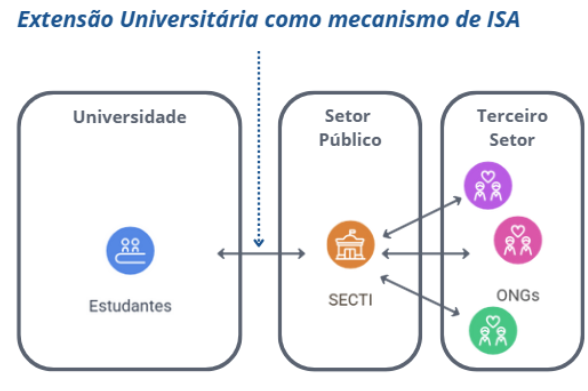
\includegraphics[width=0.6\linewidth]{images/metodologia/partesenvolvidas.png}
    \label{fig:partesenvolvidas}
    \vspace{0.2cm}

{\centering Fonte: O autor (2025). \par}
\end{figure}

Baseado no ciclo de pesquisa-ação de \citeauthor{staron2020} (\citeyear{staron2020}), o plano de pesquisa-ação, proposto nesse trabalho, constitui-se de 5 fases num período de 5 meses, como mostrado na imagem abaixo:

\begin{figure}[H]
    \caption{Ciclo de pesquisa-ação}
    \centering
    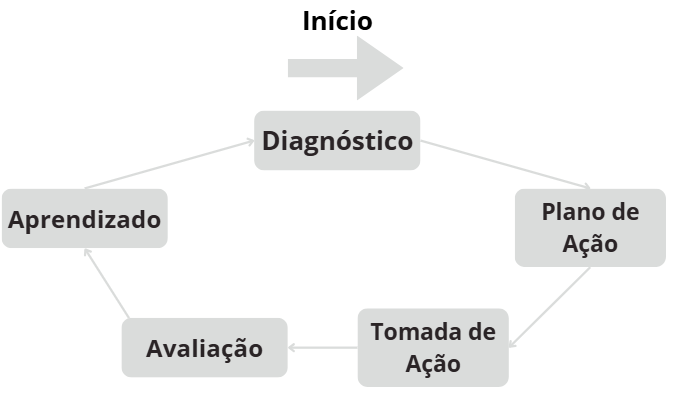
\includegraphics[width=0.5\linewidth]{images/metodologia/pesquisaacao.png}
    \label{fig:pesquisaacao}
    
    Fonte: Adaptado de \citeauthor{staron2020} (\citeyear{staron2020}, p. 3).
\end{figure}


\textbf{1. Diagnóstico — 4 semanas de duração}

Nessa seção, o atual planejamento e metodologias de execução do projeto por parte do professor serão analisados, além de uma identificação inicial das oportunidades de melhoria, focando na interação maior entre os envolvidos, possibilitando um maior processo de inovação aberta. 
Ações: 
\begin{itemize}
\item Realização de entrevistas com os estudantes e o professor acerca do que é esperado para o projeto, sua execução e seus resultados. 
\par\vspace{1\baselineskip}

\end{itemize}

\textbf{2. Plano de ação — 4 semanas de duração}

Será realizado um plano de projeto de Extensão, utilizando práticas já existentes de Inovação Social Aberta. 
Ações:
\begin{itemize}
    \item Levantamento de atores envolvidos;
    \item Criação de proposta de atividades para promover a colaboração entre os atores;
    \item Criação de cronograma proposto para intervenção.
\par\vspace{1\baselineskip}

\end{itemize}

\textbf{3. Tomada de ação —  4 semanas de duração}

Essa fase irá ser executada em uma interação mais direta com o professor e os estudantes, enquanto os mesmos estão trabalhando no processo de construção do artefato que será apresentado posteriormente. Ações:
\begin{itemize}
    \item Monitoramento do impacto sobre os \textit{stakeholders} envolvidos a respeito da execução do projeto
\par\vspace{1\baselineskip}

\end{itemize}

\textbf{4. Avaliação — 4 semanas de duração}

Essa etapa irá verificar se de fato as ações propostas causaram algum impacto sobre os atores envolvidos, e também nos artefatos produzidos pelos estudantes. Ações:
\begin{itemize}
    \item Análise do processo de pesquisa-ação até o momento;
    \item Análise dos artefatos produzidos pelos estudantes;
    \item Grupos focais e formulários com os envolvidos, sobre o processo de interação e colaboração entre os envolvidos;
    \item Identificação de possíveis melhorias.
\par\vspace{1\baselineskip}

\end{itemize}

\textbf{5. Aprendizado — 4 semanas de duração}

Nessa última fase será documentado todo o aprendizado obtido ao longo da execução da pesquisa-ação, e construção do possível processo a ser proposto. Ações:
\begin{itemize}
    \item Documentação das lições aprendidas;
    \item Documentação dos possíveis pontos de melhoria;
    \item Documentação dos impactos sobre todos os envolvidos e sobre o projeto.
\end{itemize}

